\documentclass[border=15pt]{standalone}
\usepackage{amsmath, amssymb}
\usepackage{tikz}
\usetikzlibrary{arrows.meta}

\definecolor{block0}{HTML}{E53935}
\definecolor{block1}{HTML}{1E88E5}

\begin{document}
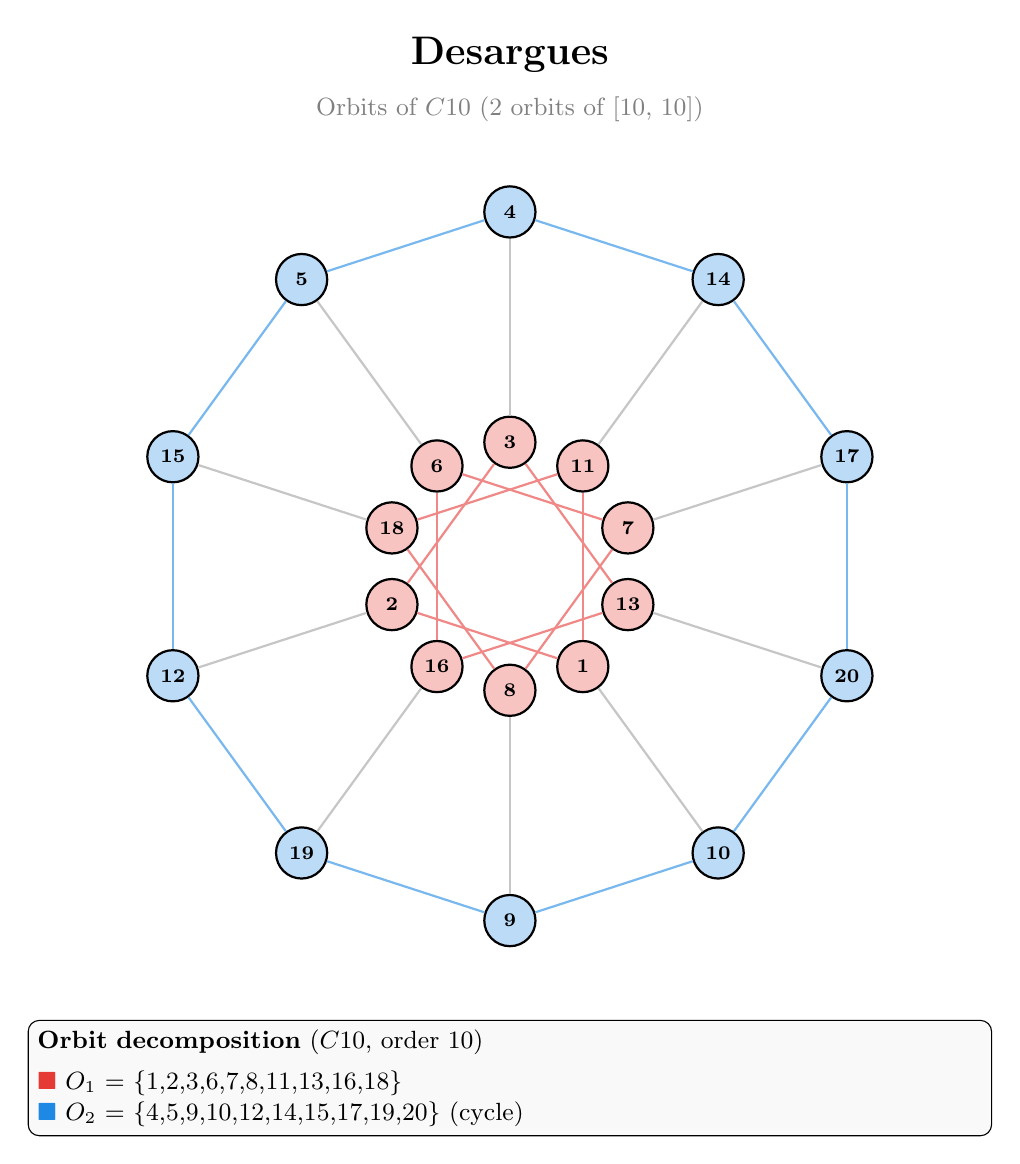
\begin{tikzpicture}[
  vertex/.style={circle, draw, thick, minimum size=6.5mm, inner sep=0pt,
                 font=\scriptsize\bfseries},
  edge/.style={thick, gray!45},
  title/.style={font=\Large\bfseries},
  subtitle/.style={font=\small, text=gray},
]

\node[title] at (0, 6.5) {Desargues};
\node[subtitle] at (0, 5.8) {Orbits of $C10$ (2 orbits of [10, 10])};

\node[vertex, fill=block0!30] (v1) at (0.926, -1.274) {1};
\node[vertex, fill=block0!30] (v2) at (-1.498, -0.487) {2};
\node[vertex, fill=block0!30] (v3) at (0.000, 1.575) {3};
\node[vertex, fill=block1!30] (v4) at (0.000, 4.500) {4};
\node[vertex, fill=block1!30] (v5) at (-2.645, 3.641) {5};
\node[vertex, fill=block0!30] (v6) at (-0.926, 1.274) {6};
\node[vertex, fill=block0!30] (v7) at (1.498, 0.487) {7};
\node[vertex, fill=block0!30] (v8) at (-0.000, -1.575) {8};
\node[vertex, fill=block1!30] (v9) at (-0.000, -4.500) {9};
\node[vertex, fill=block1!30] (v10) at (2.645, -3.641) {10};
\node[vertex, fill=block0!30] (v11) at (0.926, 1.274) {11};
\node[vertex, fill=block1!30] (v12) at (-4.280, -1.391) {12};
\node[vertex, fill=block0!30] (v13) at (1.498, -0.487) {13};
\node[vertex, fill=block1!30] (v14) at (2.645, 3.641) {14};
\node[vertex, fill=block1!30] (v15) at (-4.280, 1.391) {15};
\node[vertex, fill=block0!30] (v16) at (-0.926, -1.274) {16};
\node[vertex, fill=block1!30] (v17) at (4.280, 1.391) {17};
\node[vertex, fill=block0!30] (v18) at (-1.498, 0.487) {18};
\node[vertex, fill=block1!30] (v19) at (-2.645, -3.641) {19};
\node[vertex, fill=block1!30] (v20) at (4.280, -1.391) {20};

\draw[thick, block0!60] (v1) -- (v2);
\draw[edge] (v1) -- (v10);
\draw[thick, block0!60] (v1) -- (v11);
\draw[thick, block0!60] (v2) -- (v3);
\draw[edge] (v2) -- (v12);
\draw[edge] (v3) -- (v4);
\draw[thick, block0!60] (v3) -- (v13);
\draw[thick, block1!60] (v4) -- (v5);
\draw[thick, block1!60] (v4) -- (v14);
\draw[edge] (v5) -- (v6);
\draw[thick, block1!60] (v5) -- (v15);
\draw[thick, block0!60] (v6) -- (v7);
\draw[thick, block0!60] (v6) -- (v16);
\draw[thick, block0!60] (v7) -- (v8);
\draw[edge] (v7) -- (v17);
\draw[edge] (v8) -- (v9);
\draw[thick, block0!60] (v8) -- (v18);
\draw[thick, block1!60] (v9) -- (v10);
\draw[thick, block1!60] (v9) -- (v19);
\draw[thick, block1!60] (v10) -- (v20);
\draw[edge] (v11) -- (v14);
\draw[thick, block0!60] (v11) -- (v18);
\draw[thick, block1!60] (v12) -- (v15);
\draw[thick, block1!60] (v12) -- (v19);
\draw[thick, block0!60] (v13) -- (v16);
\draw[edge] (v13) -- (v20);
\draw[thick, block1!60] (v14) -- (v17);
\draw[edge] (v15) -- (v18);
\draw[edge] (v16) -- (v19);
\draw[thick, block1!60] (v17) -- (v20);

\node[draw, rounded corners, fill=gray!5, text width=12cm, align=left, font=\small]
  at (0, -6.5) {
  \textbf{Orbit decomposition} ($C10$, order 10) \\[4pt]
  \textcolor{block0}{$\blacksquare$} $O_{1}$ = \{1,2,3,6,7,8,11,13,16,18\} \\
  \textcolor{block1}{$\blacksquare$} $O_{2}$ = \{4,5,9,10,12,14,15,17,19,20\} (cycle)
};

\end{tikzpicture}
\end{document}